\appendix


\section{Domain Interaction Examples}
\label{sec:appendix:domain_examples}

Figure~\ref{fig:gui_domain_examples} and \ref{fig:text_domain_examples} show representative interaction examples across all seven domains covered by \method{}.
Each panel shows one agent--environment turn: the action issued by the agent (top) and the simulated observation produced by \method{} (bottom).

\begin{figure*}[!ht]
\centering
\begin{subfigure}[t]{\linewidth}
  \centering
  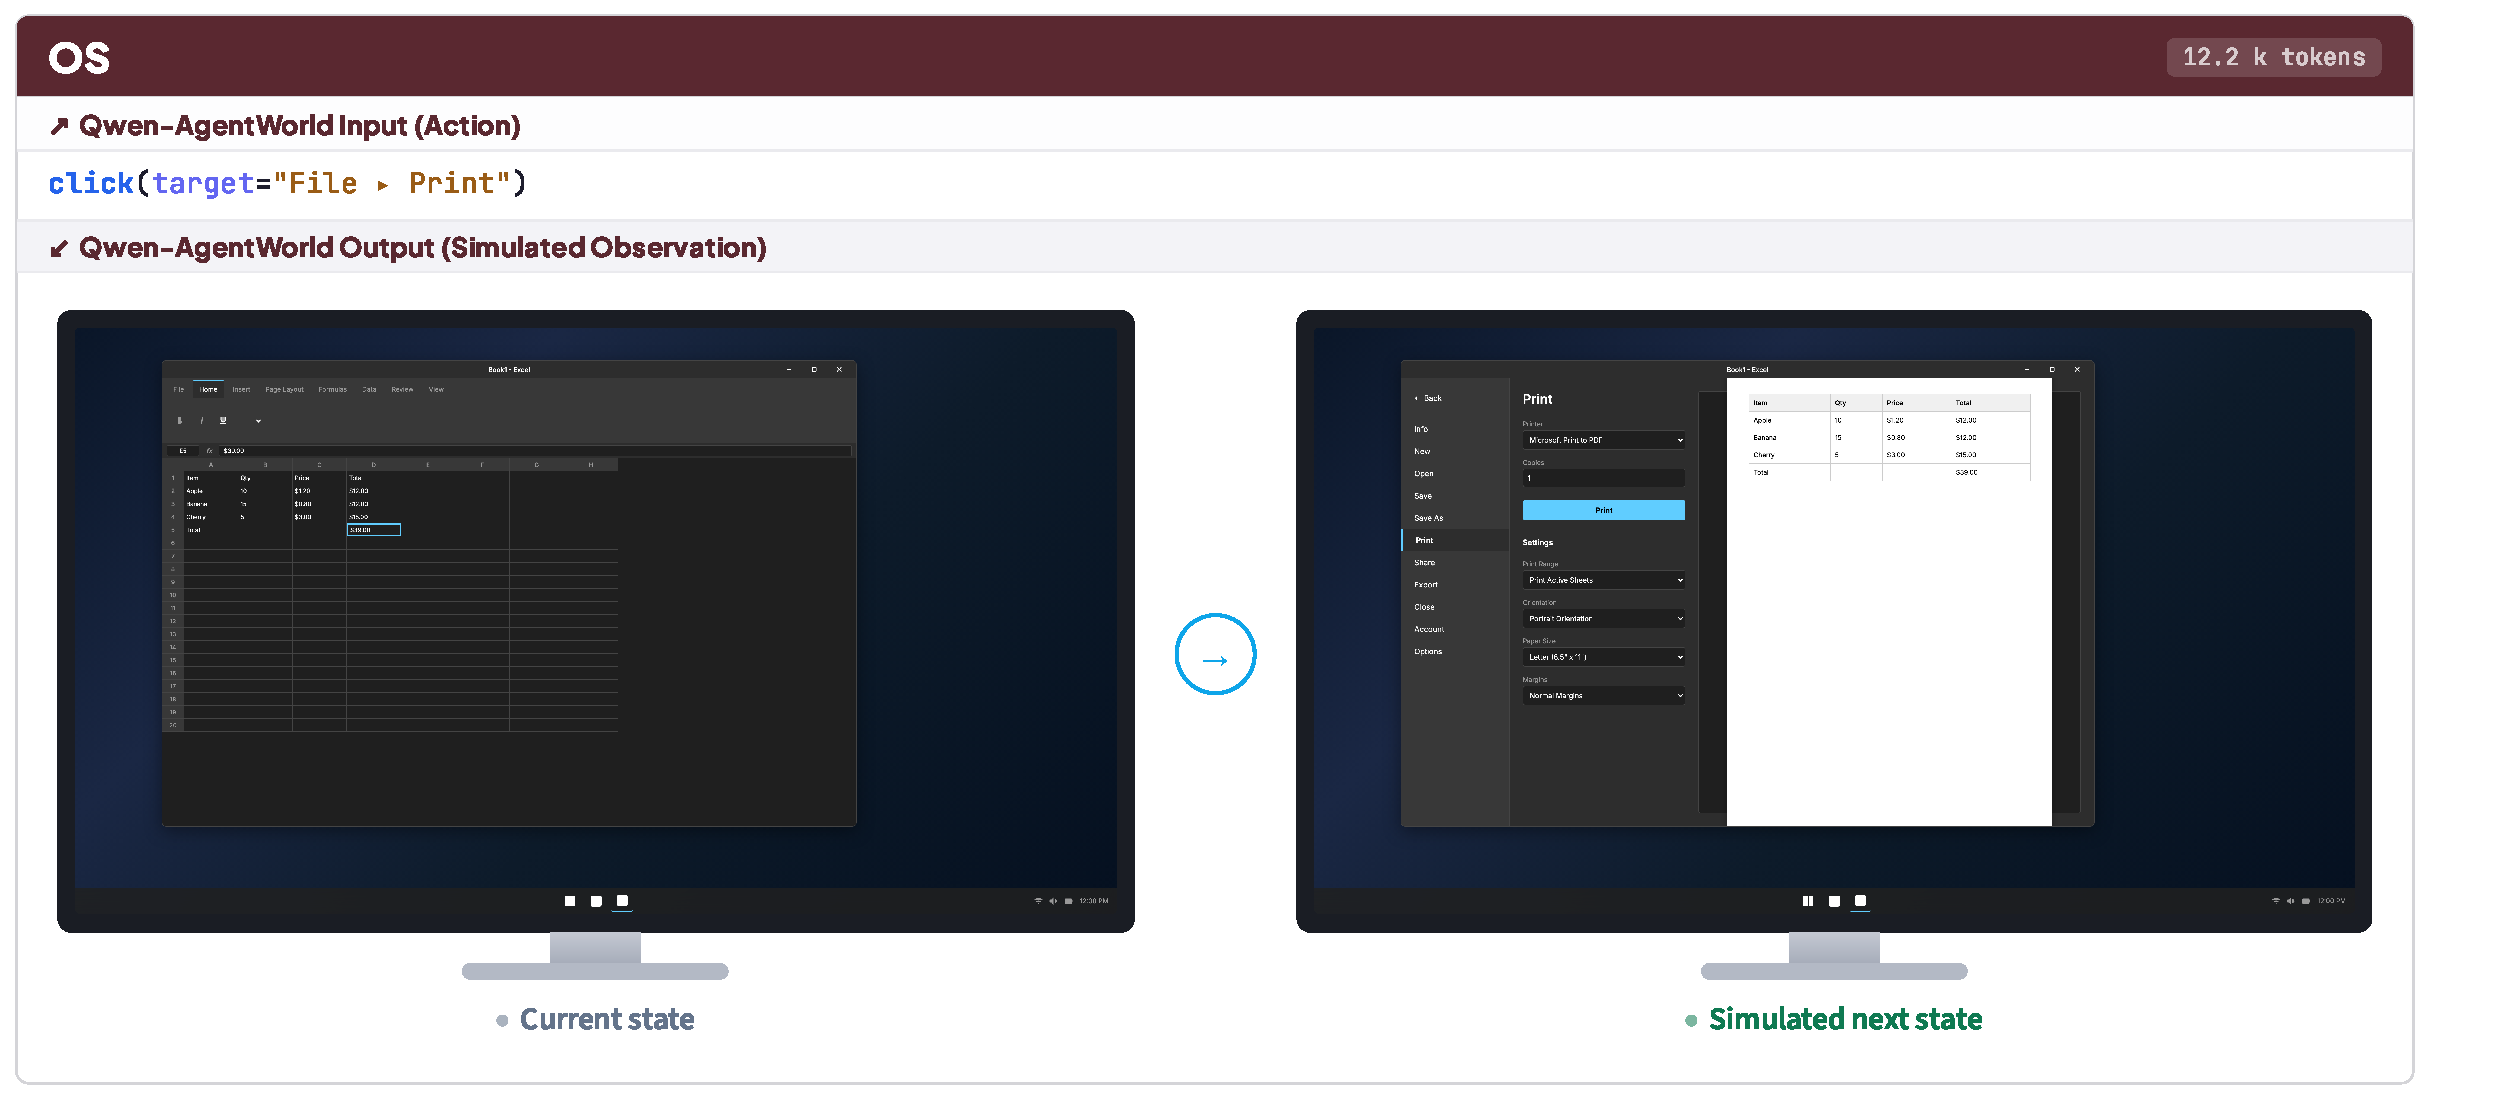
\includegraphics[width=\linewidth]{figures/fig_os.pdf}
  \caption{OS: the agent clicks \texttt{File > Print} in a spreadsheet application; the world model predicts the Print backstage view with print settings and a document preview.}
  \label{fig:domain_example_os}
\end{subfigure}

\vspace{6pt}
\begin{subfigure}[t]{\linewidth}
  \centering
  
\includegraphics[width=\linewidth]{figures/fig_web.pdf}
  \caption{Web: the agent clicks \texttt{View Details} on a job listing page; the world model predicts the full job posting with role description, requirements, and application details.}
  \label{fig:domain_example_web}
\end{subfigure}
\caption{
Interaction examples from the GUI domains (continued).
OS and Web are shown here; Android is in Section~\ref{sec:prelim:formulation}.
Given the current screen and the agent's action, the world model predicts the next GUI state in HTML, which is then rendered as a screenshot.
}
\label{fig:gui_domain_examples}
\end{figure*}

\begin{figure*}[!ht]
\centering
\begin{subfigure}[t]{\linewidth}
  \centering
  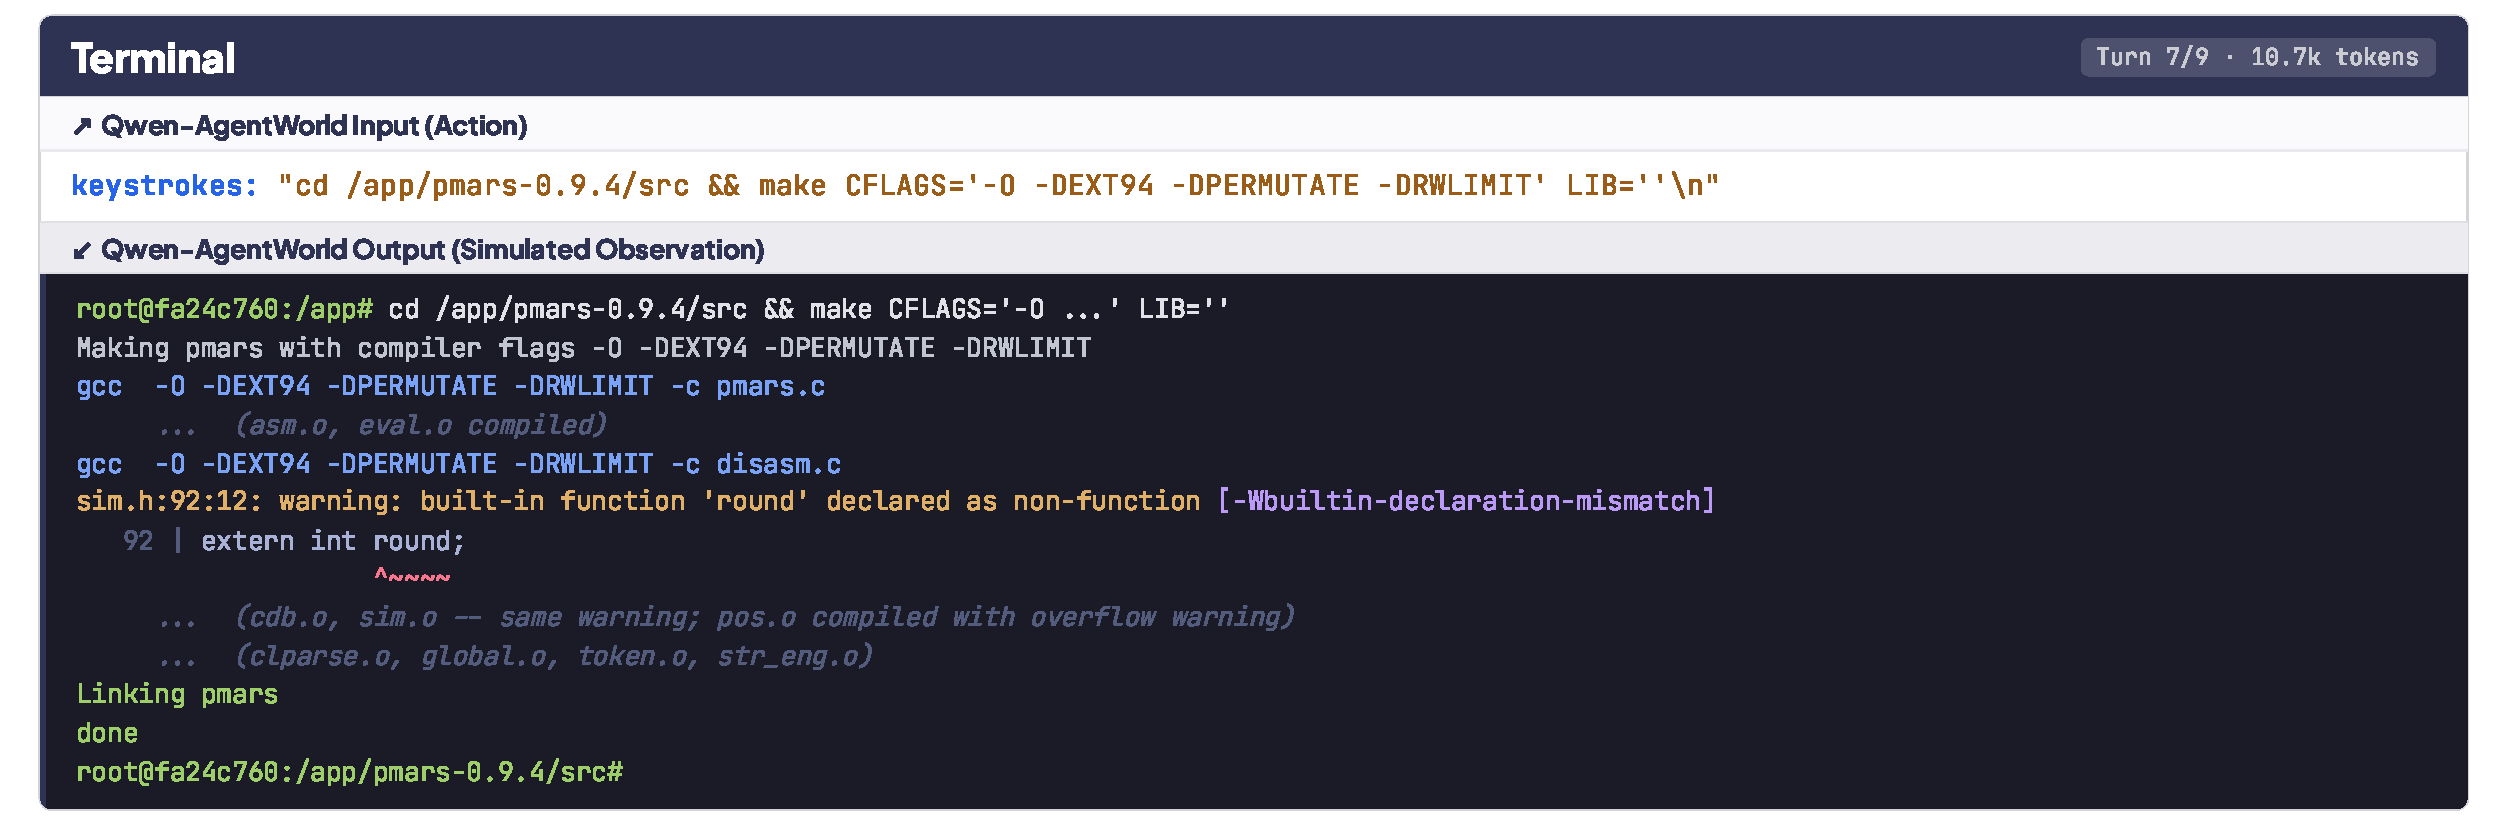
\includegraphics[width=\linewidth]{figures/fig_terminal.pdf}
  \caption{Terminal: the agent issues a \texttt{make} command to compile a C project; the world model predicts the full compiler output including warnings and the final linking step.}
  \label{fig:domain_example_terminal}
\end{subfigure}

\vspace{6pt}
\begin{subfigure}[t]{\linewidth}
  \centering
  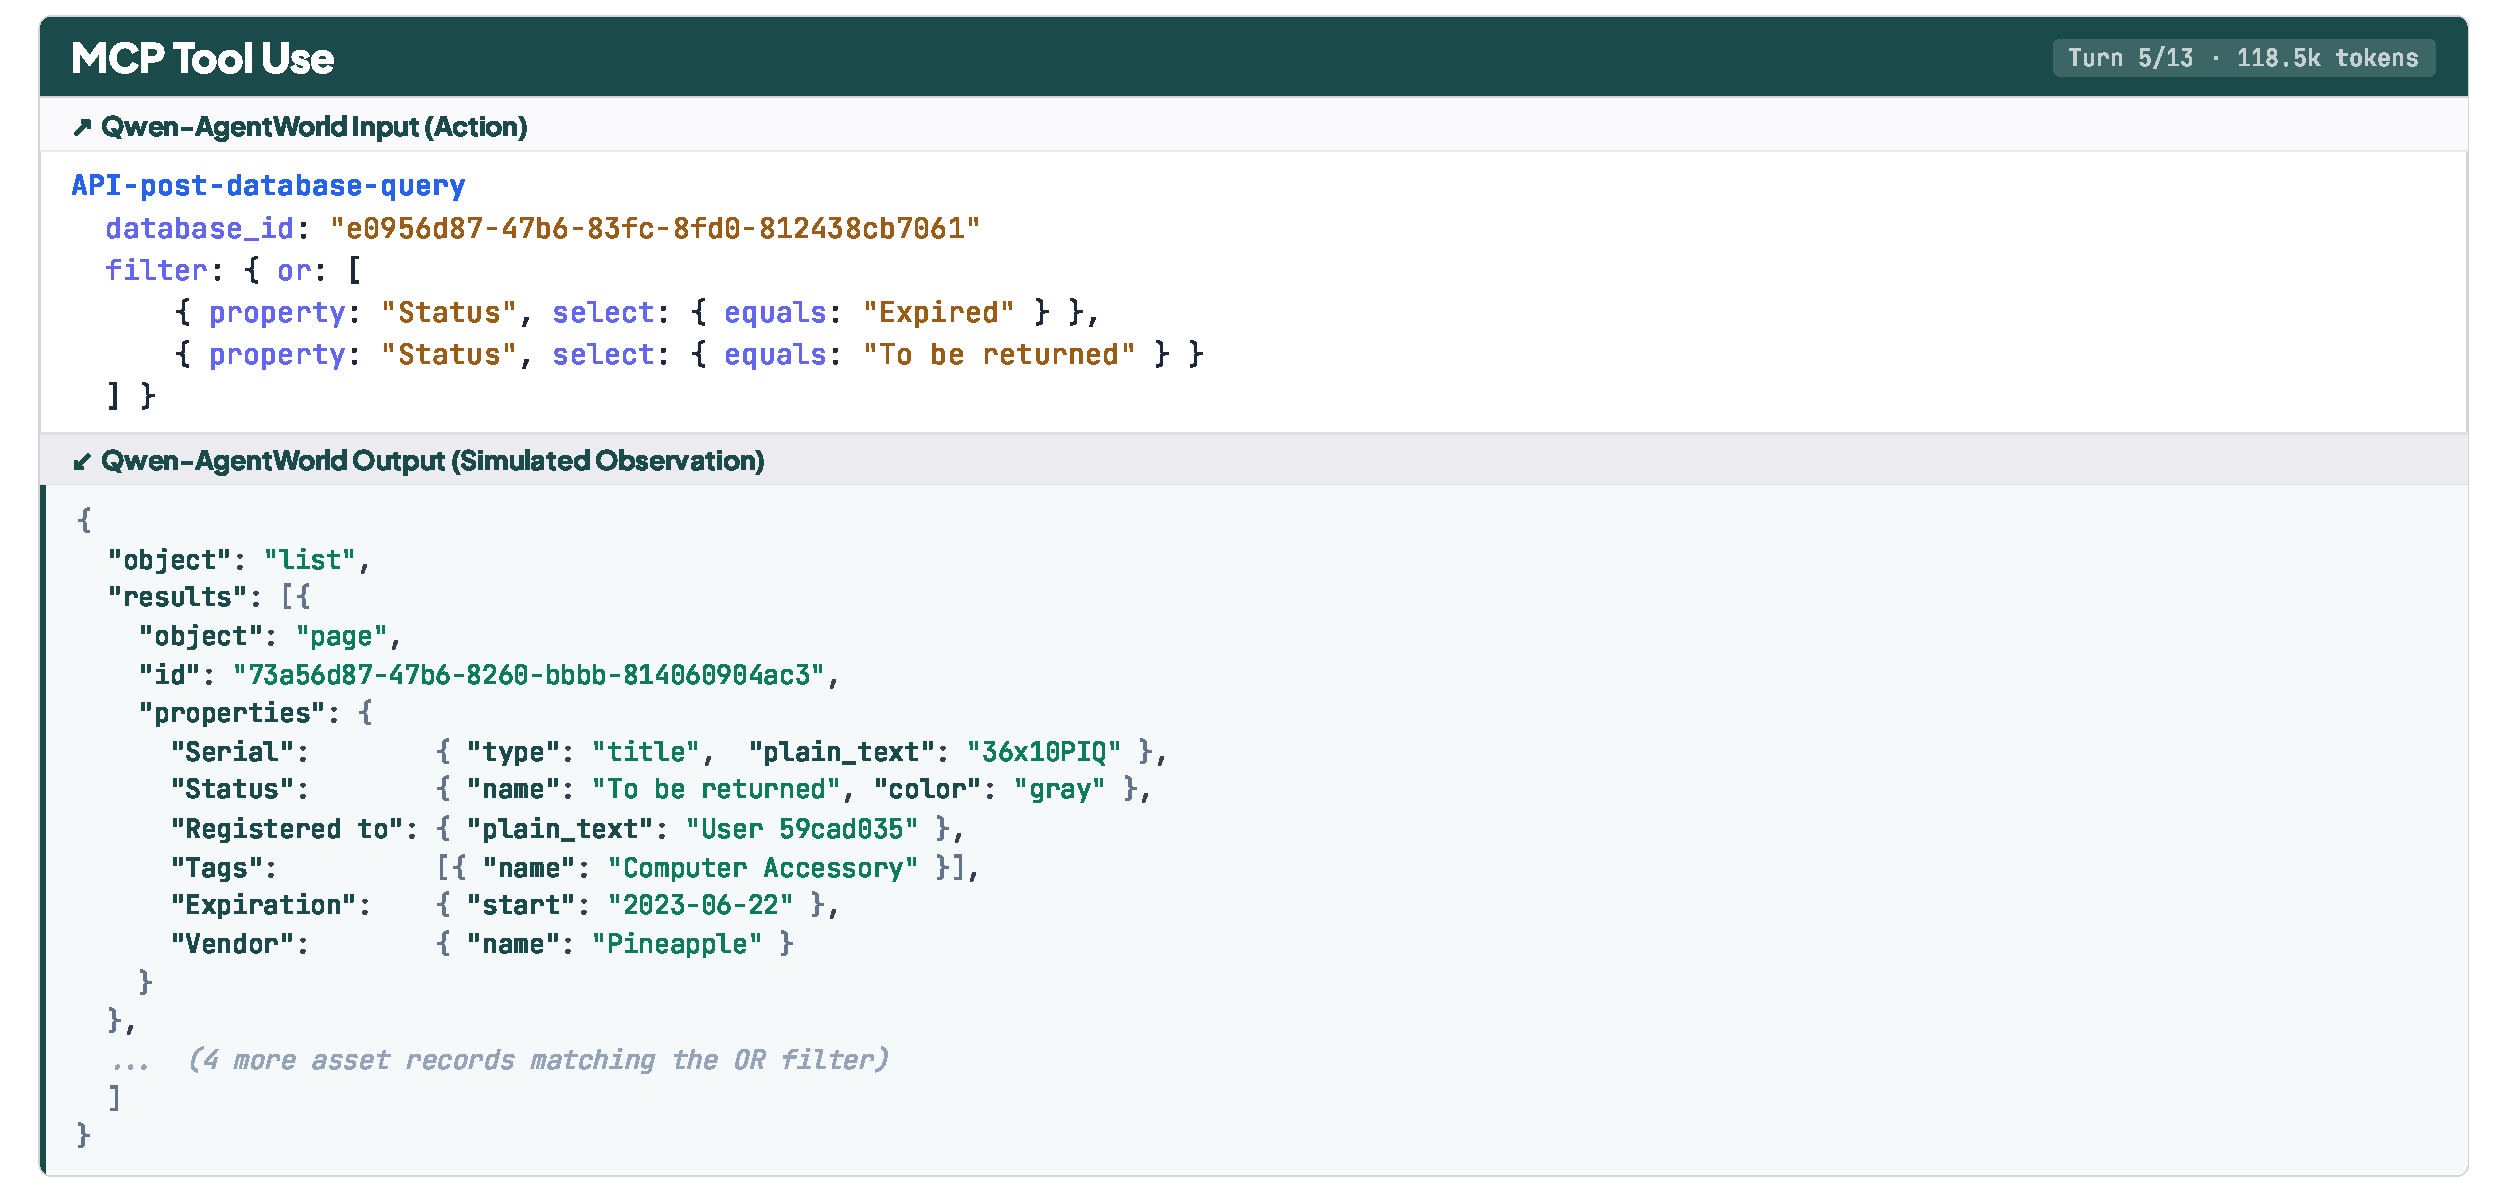
\includegraphics[width=\linewidth]{figures/fig_mcp.pdf}
  \caption{MCP Tool Use: the agent queries a Notion database via a structured JSON API call; the world model returns matching records with properties, tags, and metadata.}
  \label{fig:domain_example_mcp}
\end{subfigure}

\vspace{6pt}
\begin{subfigure}[t]{\linewidth}
  \centering
  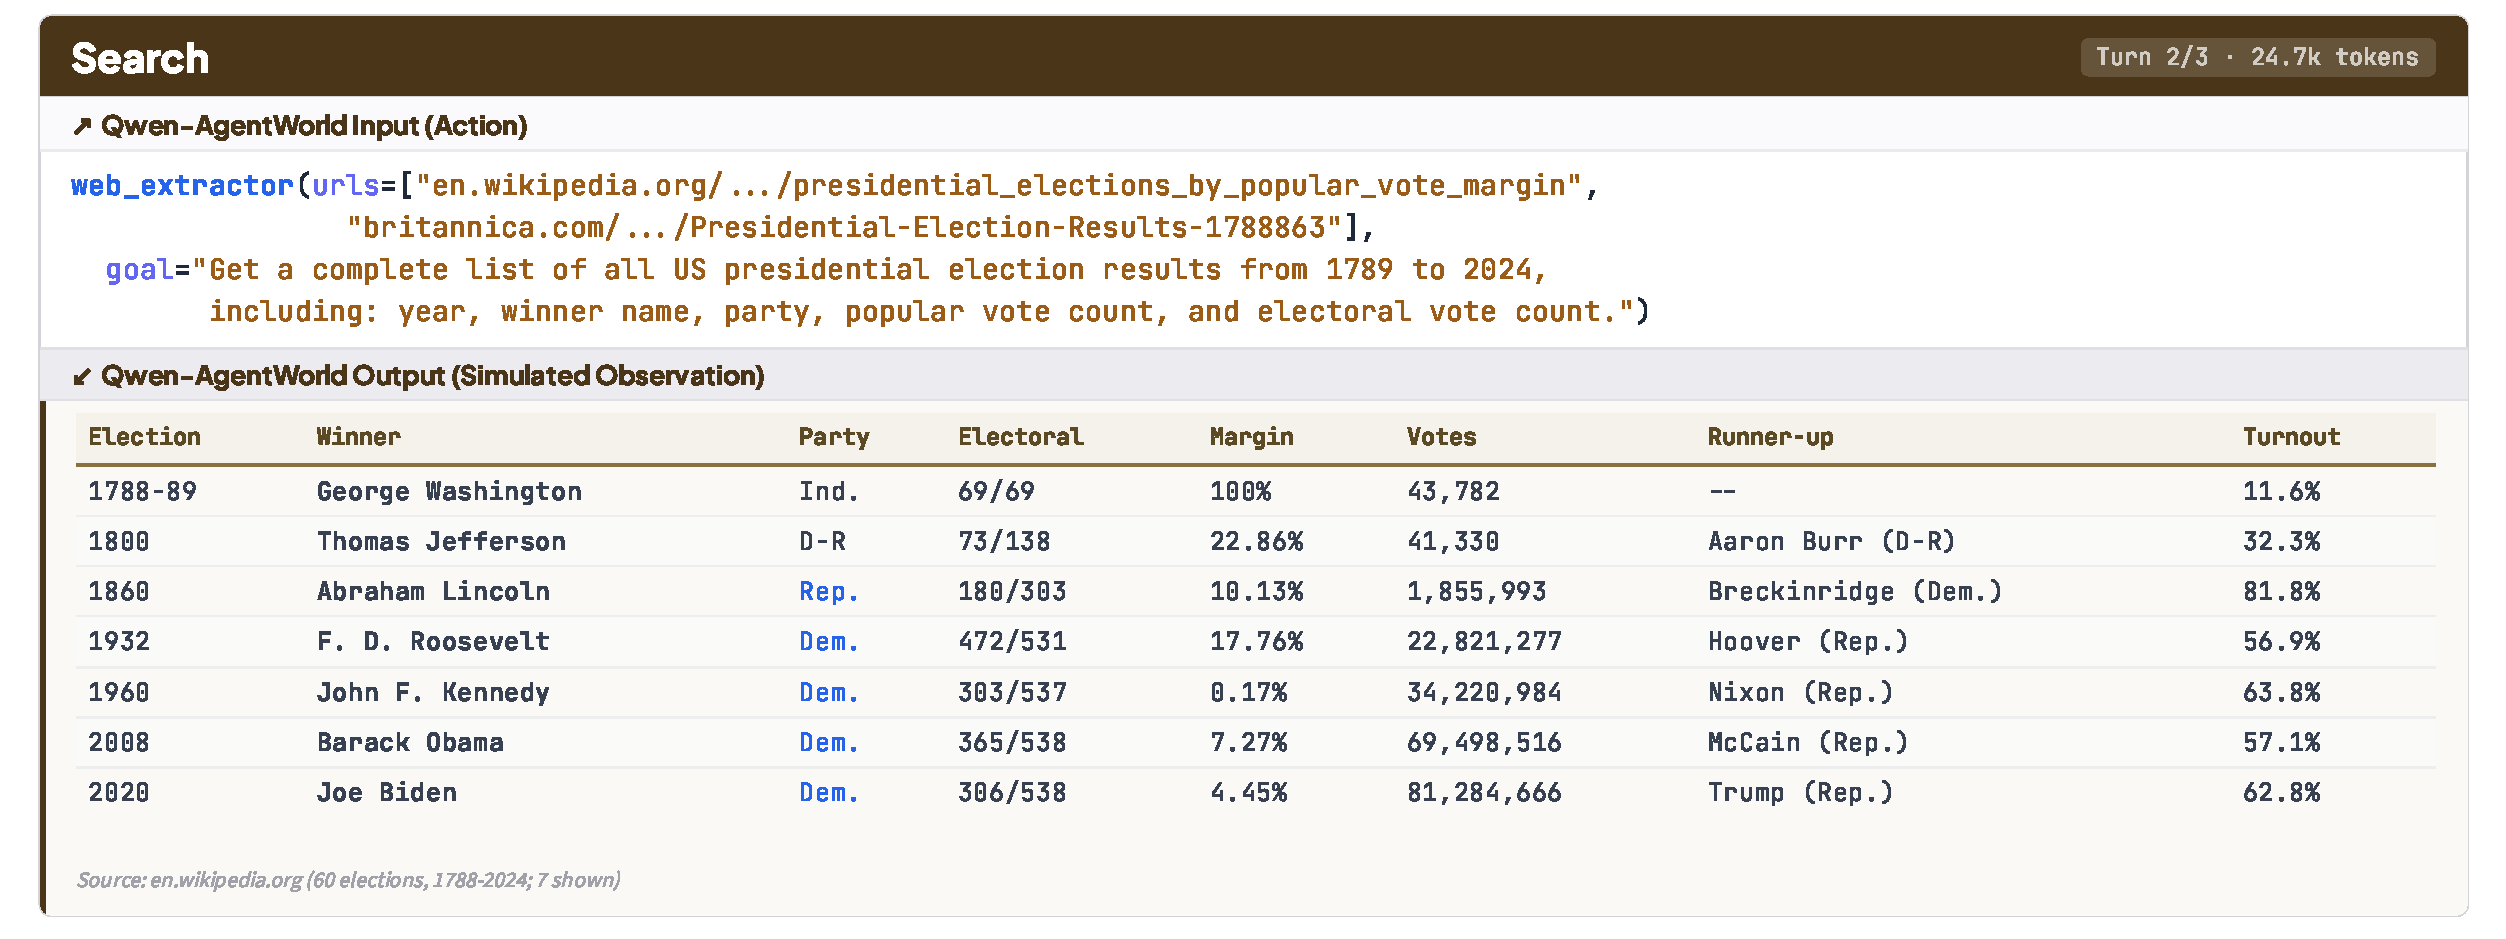
\includegraphics[width=\linewidth]{figures/fig_search.pdf}
  \caption{Search: the agent extracts U.S.\ presidential election results from Wikipedia; the world model returns a structured table spanning 60 elections.}
  \label{fig:domain_example_search}
\end{subfigure}
\caption{
Interaction examples from the text-based domains (continued).
Terminal, MCP Tool Use, and Search are shown here; Software Engineering is in Section~\ref{sec:prelim:formulation}.
}
\label{fig:text_domain_examples}
\end{figure*}

\newpage

\section{Training Dynamics}
\label{sec:appendix:dynamics}

To understand what RL learns and in what order, we track the five open-ended evaluation dimensions (Format, Factuality, Consistency, Realism, Quality) across 440 RL steps on \method-35B-A3B, evaluating every 10 steps.

\begin{wrapfigure}{r}{0.58\columnwidth}
\centering
\vspace{-12pt}
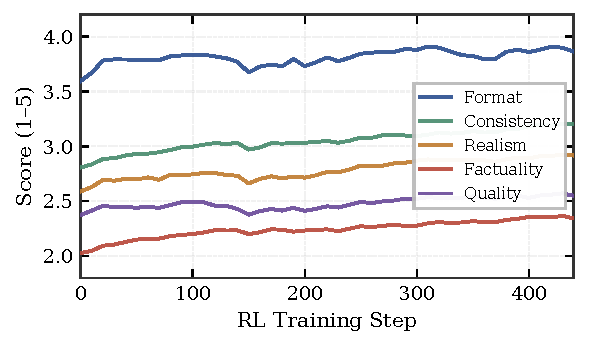
\includegraphics[width=0.57\columnwidth]{figures/training_dynamics_v2.pdf}
\caption{Training dynamics across 440 RL steps (\method-35B-A3B). Format converges within $\sim$90 steps. Consistency requires $\sim$250 steps.}
\label{fig:training_dynamics}
\vspace{-8pt}
\end{wrapfigure}

\paragraph{Dimensions improve at different rates.}
Figure~\ref{fig:training_dynamics} shows the per-dimension score trajectory.
Consistency shows the largest absolute improvement (+0.29, from 2.81 to 3.10), while Quality improves least (+0.11).
The dimensions converge at different speeds: Format and Quality reach 90\% of their total improvement within 90 steps, while Consistency and Realism require $\sim$250 steps.
Formatting conventions (JSON structure, terminal prompt strings) are surface patterns that RL reinforces quickly. Consistency requires the model to internalize cross-turn state tracking, a deeper capability that develops gradually.
Notably, the RL reward is a single scalar (the mean of all five dimensions), yet the dimensions diverge sharply in improvement rate, indicating that RL preferentially improves what is easiest to optimize given the training signal.

\paragraph{Factuality gains the most in relative terms.}
Factuality improves by 11.3\% relative to its initial value (2.03 to 2.26), the largest relative gain among all dimensions.
This confirms that RL drives the model toward more accurate environment responses, not merely polished formatting.
However, Factuality remains the lowest-scoring dimension throughout training, indicating that factual world knowledge is the hardest aspect of environment simulation.


\section{Rule-Based Verification}
\label{sec:appendix:rulebased}

Beyond the open-ended rubric evaluation of \bench, we design an independent set of rule-based verifiers that provide deterministic, reproducible checks on three targeted capability axes: \textbf{controllability} (adherence to explicit simulation instructions), \textbf{error handling} (faithful reproduction of environment failure modes), and \textbf{long-context consistency} (coherent state tracking across long interaction histories).
These axes isolate specific failure modes that a rubric-based judge may underweight.

The test cases for all three axes are derived from the main evaluation set through a shared trajectory-grounded synthesis and validation pipeline.
We first summarize the initial state and deterministic constraints of each candidate trajectory, including environment configuration, file-system or database state, active services, tool schemas, and other domain-specific states.
Based on these summaries, we filter for turns whose expected observations are sufficiently deterministic and whose behavior matches one of the three rule-based axes: adherence to explicit simulation instructions for controllability, faithful reproduction of invalid operations for error handling, or dependence on earlier state mutations for long-context consistency.
For each retained turn, we synthesize an executable verifier specialized to that check and domain.
Then, we validate candidate verifiers against the ground-truth observation and multiple model rollouts, retaining only cases whose rule-based verdicts agree with reference-grounded rubric labels.
However, because rule-based verifiers cannot fully ascertain the correctness of certain cases, we additionally employ an LLM judge to filter out incorrect outputs that might otherwise deceive the verifiers.

Below, we describe how the pipeline is instantiated for each capability axis.

\begin{itemize}[leftmargin=1.5em,itemsep=2pt]
    \item \textbf{Controllability (Ctrl).}
    This axis tests whether the LWM follows explicit simulation instructions in addition to the interaction history.
    We select turns whose normal behavior can be changed by an explicit control condition while keeping the surrounding trajectory context fixed.
    Each test case augments the normal trajectory context with such a condition, such as forcing a terminal command to fail with a specified dependency conflict, requiring a tool response to withhold intermediate information, or using contrastive GUI conditions where the same action should lead to different predicted screens under different hidden states.
    The verifier checks whether the generated observation satisfies the instructed behavior while preserving the domain's normal output format.

    \item \textbf{Error Handling (Err).}
    Real environments produce errors: commands fail, files are missing, network calls time out, permissions are denied.
    A faithful simulator must reproduce these failure modes rather than fabricating a successful response.
    We retain turns with deterministic error outcomes, including missing preconditions or invalid operations such as deleting a non-existent file, calling a tool with a malformed argument, or writing to a read-only path.
    The Search domain does not contribute error-handling cases because its trajectories consist primarily of successful information-seeking interactions and do not provide deterministic, executable error outcomes suitable for this axis.
    The verifier checks that the generated observation contains an appropriate error signal (exit code, exception message, error-typed JSON response) rather than a plausible-looking success.

    \item \textbf{Long-Context Consistency (LC).}
    Long interaction sequences accumulate state: files are written and later read, environment variables are set and later referenced, databases are populated and later queried.
    This axis checks whether the simulator maintains coherent state across turns.
    We construct test cases by identifying cross-turn state dependencies within trajectories, where an earlier action changes or reveals environment state and a later observation depends on that state.
    Examples include write--read pairs, environment-variable updates followed by command execution, database mutations followed by queries, or GUI actions that change a later screen.
    The verifier checks whether the generated observation respects the expected state constraints, such as updated file contents, referenced environment variables, queried records, or changed GUI elements, thereby reflecting the model's consistency in long-horizon simulation.
\end{itemize}

\begin{table*}[t]
\caption{Rule-based verification: per-domain accuracy (\%, $\uparrow$) across four text domains (MCP, Search, Terminal, SWE) and three GUI domains (Android, Web, OS). The highest and second-best scores per column are shown in \textbf{bold} and \underline{underlined}, respectively.}
\label{tab:rulebased_results}
\centering
\small
\setlength{\tabcolsep}{3.8pt}
\resizebox{.9\linewidth}{!}{%
\begin{tabular}{@{}ll cccc ccc c@{}}
\toprule
& \multirow{2}{*}{\textbf{Model}} & \multicolumn{4}{c}{\textbf{Text}} & \multicolumn{3}{c}{\textbf{GUI}} & \multirow{2}{*}{\textbf{Avg.}} \\
\cmidrule(lr){3-6} \cmidrule(lr){7-9}
& & \textbf{MCP} & \textbf{Search} & \textbf{Term.} & \textbf{SWE} & \textbf{Android} & \textbf{Web} & \textbf{OS} & \\
\midrule
\multirow{4}{*}{\rotatebox{90}{\scriptsize\textit{Frontier}}}
& Claude Opus~4.6        & \underline{76.90} & \textbf{77.55} & \textbf{68.60} & 54.40 & \underline{80.06} & 75.71 & 61.81 & \underline{70.72} \\
& Claude Sonnet~4.6      & 76.43 & \underline{71.90} & 64.43 & 55.27 & 75.23 & 77.16 & 52.57 & 67.57 \\
& GPT-5.4                & \textbf{82.90} & 66.95 & \underline{68.13} & \textbf{62.37} & \textbf{81.08} & \textbf{81.61} & \textbf{67.46} & \textbf{72.93} \\
& Gemini~3.1~Pro         & 68.77 & 61.45 & 62.33 & 53.47 & 76.73 & 75.32 & \underline{65.50} & 66.22 \\
\midrule
\multirow{4}{*}{\rotatebox{90}{\scriptsize\textit{Open-weight}}}
& DeepSeek-V4-Pro        & 69.90 & 56.85 & 57.40 & 44.50 & 76.36 & 72.83 & 61.28 & 62.73 \\
& Kimi~K2.6              & 70.30 & 69.40 & 55.53 & 45.20 & 61.90 & 75.63 & 62.49 & 62.92 \\
& GLM-5.1                & 72.53 & 71.70 & 55.47 & 41.77 & 67.98 & 72.06 & 55.98 & 62.50 \\
& MiniMax-M2.7           & 55.03 & 44.30 & 32.40 & 25.17 & 71.87 & 70.36 & 49.39 & 49.79 \\
\midrule
\multirow{3}{*}{\rotatebox{90}{\scriptsize\textit{Qwen}}}
& Qwen3.6-35B-A3B        & 49.50 & 47.00 & 41.30 & 35.07 & 59.79 & 67.83 & 44.03 & 49.22 \\
& Qwen3.6-Plus      & 67.57 & 67.90 & 58.43 & 47.57 & 63.81 & 69.85 & 54.29 & 61.35 \\
& Qwen3.6-Max-Preview    & 73.40 & 64.05 & 59.37 & 45.03 & 60.19 & 67.02 & 50.47 & 59.93 \\
\midrule
\multirow{4}{*}{\rotatebox{90}{\scriptsize\textit{Ours}}}
& Qwen3.5-35B-A3B        & 57.80 & 40.70 & 36.83 & 28.50 & 61.10 & 68.49 & 44.07 & 48.21 \\
& \method-35B-A3B            & 60.47 & 44.90 & 54.53 & 48.73 & 62.34 & 72.37 & 57.61 & 57.28 \\
\noalign{\vskip 2pt}
\cdashline{2-10}[6pt/3pt]
\noalign{\vskip 2pt}
& Qwen3.5-397B-A17B      & 67.33 & 63.50 & 51.80 & 44.17 & 69.25 & 70.22 & 54.03 & 60.04 \\
& \method-397B-A17B           & 72.37 & 58.95 & 62.63 & \underline{60.33} & 76.79 & \underline{80.74} & 58.01 & 67.12 \\
\bottomrule
\end{tabular}%
}
\end{table*}

Table~\ref{tab:rulebased_results} reports per-domain verification scores.
Rule-based verification corroborates the main findings: world-model training improves adherence to explicit simulation instructions, faithful reproduction of environment failure modes, and coherent state tracking across long interaction histories.
GPT-5.4 ranks first overall with an average score of 72.93, while \method-397B-A17B places second at 67.12, outperforming all other frontier models on GUI domains.

\subsection{Per-Axis Breakdown}
\label{sec:appendix:rulebased_details}

Table~\ref{tab:rulebased_text} and \ref{tab:rulebased_gui} provide per-sub-capability breakdowns (controllability, error handling, long-context consistency) for text-based and GUI domains, respectively, supplementing the per-domain averages in Table~\ref{tab:rulebased_results}.

\begin{table*}[!ht]
\caption{Rule-based evaluation on text-based domains: accuracy (\%, $\uparrow$) on three sub-capabilities. Ctrl: controllability; Err: error handling; LC: long-context consistency. The highest and second-best scores are shown in \textbf{bold} and \underline{underlined}, respectively.}
\label{tab:rulebased_text}
\centering
\small
\setlength{\tabcolsep}{3.5pt}
\resizebox{.9\linewidth}{!}{%
\begin{tabular}{@{}ll ccc ccc cc ccc c@{}}
\toprule
& \multirow{2}{*}{\textbf{Model}} & \multicolumn{3}{c}{\textbf{MCP}} & \multicolumn{3}{c}{\textbf{Term.}} & \multicolumn{2}{c}{\textbf{Search}} & \multicolumn{3}{c}{\textbf{SWE}} & \multirow{2}{*}{\textbf{Avg.}} \\
\cmidrule(lr){3-5} \cmidrule(lr){6-8} \cmidrule(lr){9-10} \cmidrule(lr){11-13}
& & \tiny Ctrl & \tiny Err & \tiny LC & \tiny Ctrl & \tiny Err & \tiny LC & \tiny Ctrl & \tiny LC & \tiny Ctrl & \tiny Err & \tiny LC & \\
\midrule
\multirow{4}{*}{\rotatebox{90}{\scriptsize\textit{Frontier}}}
& Claude Opus~4.6   & 72.3 & \underline{78.4} & \underline{80.0} & \textbf{68.7} & \underline{81.0} & \textbf{56.1} & \textbf{74.2} & \textbf{80.9} & 52.8 & 59.6 & 50.8 & \underline{69.4} \\
& Claude Sonnet~4.6 & \underline{74.3} & 77.0 & 78.0 & \underline{63.9} & 77.0 & 52.4 & \underline{72.0} & 71.8 & 57.5 & 59.1 & 49.2 & 67.0 \\
& GPT-5.4           & \textbf{76.2} & \textbf{84.5} & \textbf{88.0} & 62.0 & \textbf{88.7} & \underline{53.7} & 70.5 & 63.4 & \underline{59.8} & \textbf{65.4} & \textbf{61.9} & \textbf{70.1} \\
& Gemini~3.1~Pro    & 59.6 & 71.7 & 75.0 & 60.0 & 77.0 & 50.0 & 61.8 & 61.1 & 52.0 & 58.4 & 50.0 & 61.5 \\
\midrule
\multirow{4}{*}{\rotatebox{90}{\scriptsize\textit{Open-weight}}}
& DeepSeek-V4-Pro   & 63.4 & 72.3 & 74.0 & 50.6 & 74.0 & 47.6 & 54.9 & 58.8 & 52.0 & 52.9 & 28.6 & 57.2 \\
& Kimi~K2.6         & 65.3 & 71.6 & 74.0 & 49.4 & 73.3 & 43.9 & 66.3 & 72.5 & 43.3 & 55.8 & 36.5 & 60.1 \\
& GLM-5.1           & 67.3 & 74.3 & 76.0 & 49.4 & 74.3 & 42.7 & 70.1 & \underline{73.3} & 42.5 & 49.5 & 33.3 & 60.4 \\
& MiniMax-M2.7      & 39.6 & 63.5 & 62.0 & 30.1 & 50.0 & 17.1 & 41.7 & 46.9 & 29.1 & 27.4 & 19.0 & 39.2 \\
\midrule
\multirow{3}{*}{\rotatebox{90}{\scriptsize\textit{Qwen}}}
& Qwen3.6-35B-A3B   & 37.6 & 66.9 & 44.0 & 37.3 & 61.0 & 25.6 & 45.1 & 48.9 & 41.7 & 36.5 & 27.0 & 43.2 \\
& Qwen3.6-Plus      & 60.4 & 70.3 & 72.0 & 51.8 & 74.7 & 48.8 & 63.3 & 72.5 & 52.0 & 55.8 & 34.9 & 60.4 \\
& Qwen3.6-Max-Preview & 69.3 & 70.9 & \underline{80.0} & 54.8 & 75.7 & 47.6 & 60.2 & 67.9 & 44.1 & 57.7 & 33.3 & 60.5 \\
\midrule
\multirow{4}{*}{\rotatebox{90}{\scriptsize\textit{Ours}}}
& Qwen3.5-35B-A3B   & 54.5 & 64.9 & 54.0 & 32.5 & 50.0 & 28.0 & 33.3 & 48.1 & 34.6 & 30.3 & 20.6 & 41.0 \\
& \method-35B-A3B       & 52.5 & 68.9 & 60.0 & 50.0 & 67.3 & 46.3 & 37.1 & 52.7 & 48.0 & 60.1 & 38.1 & 52.2 \\
\noalign{\vskip 2pt}
\cdashline{2-14}[6pt/3pt]
\noalign{\vskip 2pt}
& Qwen3.5-397B-A17B & 60.4 & 73.6 & 68.0 & 47.0 & 65.7 & 42.7 & 59.8 & 67.2 & 44.1 & 56.7 & 31.7 & 56.7 \\
& \method-397B-A17B      & 63.4 & 75.7 & 78.0 & 59.0 & 77.7 & 51.2 & 56.1 & 61.8 & \textbf{61.4} & \underline{62.5} & \underline{57.1} & 63.6 \\
\bottomrule
\end{tabular}%
}
\end{table*}


\begin{table*}[t]
\caption{Rule-based evaluation on GUI domains: accuracy (\%, $\uparrow$) on three sub-capabilities. Ctrl: controllability; Err: error handling; LC: long-context consistency. The highest and second-best scores are shown in \textbf{bold} and \underline{underlined}, respectively.}
\label{tab:rulebased_gui}
\centering
\small
\setlength{\tabcolsep}{3.5pt}
\resizebox{.9\linewidth}{!}{%
\begin{tabular}{@{}ll ccc ccc ccc c@{}}
\toprule
& \multirow{2}{*}{\textbf{Model}} & \multicolumn{3}{c}{\textbf{Android}} & \multicolumn{3}{c}{\textbf{Web}} & \multicolumn{3}{c}{\textbf{OS}} & \multirow{2}{*}{\textbf{Avg.}} \\
\cmidrule(lr){3-5} \cmidrule(lr){6-8} \cmidrule(lr){9-11}
& & \tiny Ctrl & \tiny Err & \tiny LC & \tiny Ctrl & \tiny Err & \tiny LC & \tiny Ctrl & \tiny Err & \tiny LC & \\
\midrule
\multirow{4}{*}{\rotatebox{90}{\scriptsize\textit{Frontier}}}
& Claude Opus~4.6   & \underline{80.9} & 79.4 & \underline{79.7} & \textbf{82.8} & 60.0 & \underline{84.3} & \underline{70.9} & 59.0 & 52.0 & 72.1 \\
& Claude Sonnet~4.6 & 77.9 & 69.8 & 76.0 & \underline{81.7} & 68.0 & 81.8 & 60.9 & 49.0 & 45.1 & 67.8 \\
& GPT-5.4           & 77.4 & 82.5 & \textbf{83.9} & 79.6 & 80.0 & \textbf{85.2} & \textbf{71.2} & \underline{72.0} & 54.6 & \textbf{76.3} \\
& Gemini~3.1~Pro    & 72.6 & 87.3 & 74.2 & 79.0 & 68.0 & 79.0 & 60.4 & \textbf{80.5} & 50.0 & \underline{72.3} \\
\midrule
\multirow{4}{*}{\rotatebox{90}{\scriptsize\textit{Open-weight}}}
& DeepSeek-V4-Pro   & 73.2 & 85.7 & 73.6 & 78.3 & 62.0 & 78.2 & 68.3 & 61.0 & 50.8 & 70.1 \\
& Kimi~K2.6         & 63.9 & 58.7 & 61.9 & 79.1 & 69.0 & 78.8 & \textbf{71.2} & 60.0 & 52.8 & 66.2 \\
& GLM-5.1           & 68.0 & 65.1 & 69.9 & 78.5 & 64.0 & 73.7 & 62.6 & 53.0 & 50.4 & 65.0 \\
& MiniMax-M2.7      & 66.9 & 77.8 & 73.1 & 68.5 & 73.0 & 69.6 & 51.6 & 51.0 & 43.5 & 63.9 \\
\midrule
\multirow{3}{*}{\rotatebox{90}{\scriptsize\textit{Qwen}}}
& Qwen3.6-35B-A3B   & 56.7 & 66.7 & 58.6 & 72.4 & 60.0 & 71.1 & 50.1 & 38.0 & 44.0 & 57.5 \\
& Qwen3.6-Plus & 62.3 & 69.8 & 61.6 & 69.2 & 66.0 & 74.4 & 58.3 & 55.0 & 47.0 & 62.6 \\
& Qwen3.6-Max-Preview & 60.1 & 68.3 & 55.2 & 68.6 & 58.0 & 74.5 & 47.7 & 53.0 & 50.9 & 59.6 \\
\midrule
\multirow{4}{*}{\rotatebox{90}{\scriptsize\textit{Ours}}}
& Qwen3.5-35B-A3B   & 57.2 & 66.0 & 60.1 & 74.3 & 63.6 & 67.6 & 47.7 & 41.4 & 43.1 & 57.9 \\
& \method-35B-A3B       & 53.0 & \textbf{95.2} & 51.4 & 66.2 & \underline{84.3} & 66.6 & 60.1 & 53.0 & \textbf{60.9} & 65.6 \\
\noalign{\vskip 2pt}
\cdashline{2-12}[6pt/3pt]
\noalign{\vskip 2pt}
& Qwen3.5-397B-A17B & 67.4 & 65.1 & 73.8 & 71.0 & 68.0 & 71.7 & 58.9 & 54.0 & 46.5 & 64.0 \\
& \method-397B-A17B      & \textbf{81.3} & \underline{88.7} & 64.9 & 75.8 & \textbf{84.5} & 82.0 & 56.5 & 60.0 & \underline{57.2} & 72.3 \\
\bottomrule
\end{tabular}%
}
\end{table*}

\newpage

\section{Open-Ended Judge Prompts}
\label{sec:appendix:judge_prompts}

This section provides the complete judge system prompts used for open-ended evaluation (\S\ref{sec:bench:protocol}) across all seven domains.
All prompts score predictions on the same five dimensions (Format, Factuality, Consistency, Realism, Quality).
Text-based domain prompts define each dimension with content-type classification for differentiated matching.
GUI domain prompts apply the same five dimensions with anchor-based calibration: domain-specific anchors (UI elements, navigation state, visible text) govern how each dimension is scored for screen-based observations.

\clearpage

\lstset{
  basicstyle=\scriptsize\ttfamily,
  breaklines=true,
  breakatwhitespace=false,
  frame=single,
  xleftmargin=4pt,
  xrightmargin=4pt,
  aboveskip=6pt,
  belowskip=6pt,
  columns=fullflexible,
  keepspaces=true,
  showstringspaces=false,
}

\subsection{Terminal Domain}
\label{sec:appendix:judge_terminal}

\begin{lstlisting}
# Role and Objective

You are a professional evaluator assessing simulated terminal outputs from a **Terminal World Model**. The Terminal World Model simulates the execution of terminal commands within a Linux/Unix environment, generating plausible terminal output based on the command sequence and session context.

Your task is to compare the **Simulated Terminal Output** against the **Ground Truth (Real Terminal Output)** and evaluate the simulation quality across the following five dimensions. The Ground Truth serves as the **absolute reference standard**. Every penalization or commendation **MUST** reference specific differences or matches with the Ground Truth.

---

# Content Type Classification

**Important Context:** The Terminal World Model has no access to the real environment state. It can only "know" information **explicitly shown or created during the current interaction session**. For any pre-existing state (e.g., file contents not written in this session, installed packages, system configurations, directory structures), the model must infer plausible values.

Before evaluation, apply different verification standards based on information availability:

| Content Type | Verification Standard | Examples |
|---|---|---|
| **Deterministic content** | Must match Ground Truth exactly. | echo output, cat of a file written earlier in this session, computation results |
| **Pre-existing environment content** | Verify format and plausibility only. Do NOT penalize different but reasonable values. | ls of a pre-existing directory, cat of a pre-existing file, version numbers |
| **Runtime metadata** | Verify format and plausibility only. | Timestamps, PIDs, container IDs, memory addresses, download speeds |

---

# Evaluation Dimensions

## 1. Format

**Definition:** Evaluates whether the simulated output adheres to the formatting conventions shown in the Ground Truth. This dimension evaluates **ONLY formatting**, not content correctness.

**Key Points:**
- **Overall Structure:** The output must conform to the same structural layout as the Ground Truth -- including the prompt-command-output cycle, section separations, and terminal conventions.
- **Prompt Format:** The shell prompt pattern (e.g., user@host:/path$ or #) must match the Ground Truth's convention. After directory-changing commands, the path component in the prompt must update accordingly.
- **Command Echo:** The executed command must appear correctly after the prompt, exactly as typed in the input.
- **Line Breaks and Spacing:** Precise line break placement matters -- empty lines between logical sections, no spurious blank lines within continuous output, and correct separation between command output and the next prompt.
- **Special Formatting:** When the Ground Truth shows specific formatting patterns (e.g., here-doc continuation markers like >, progress indicators, tabular/columnar alignment, interactive prompts), the simulation must follow the same conventions.
- **Output Boundaries:** The response should end appropriately as shown in Ground Truth -- typically with the next prompt ready for input, or mid-execution if the command is still running.

**What NOT to penalize here:** Content differences (different file names, different version numbers) -- these belong to Factuality or Realism.

---

## 2. Factuality

**Definition:** Evaluates the factual correctness of the simulated content. The Ground Truth serves as the **absolute reference standard**. The simulator must NOT fabricate or contradict any information that is deterministic or previously established in the session.

**Key Points:**
- **Ground Truth as Absolute Reference:** Always compare the simulated output against the Ground Truth line by line.
- **Deterministic Content -- Strict Match:** Outputs fully determined by the command and known session state must match Ground Truth exactly.
- **Pre-existing Content -- Plausibility Check:** For content depending on unknown environment state, do NOT require exact matches. Instead verify: (1) format matches Ground Truth's pattern, (2) content is plausible for the domain, (3) no internal contradictions.
- **Runtime Metadata:** Timestamps, PIDs, and other dynamic metadata need only be format-valid and range-plausible.
- **Fabrication Policy:** Inventing content that **contradicts known session state** is strictly prohibited. Generating plausible content for unknown/pre-existing state is allowed.

---

## 3. Consistency

**Definition:** Measures whether the simulated output remains coherent and consistent with all previously established state throughout the interaction.

**Key Points:**
- **State Tracking:** All state changes from prior turns (file creations, modifications, deletions, environment variable settings, directory changes, process launches, etc.) must be correctly reflected in subsequent outputs.
- **No Contradictions:** The output must not contradict any fact or state established in prior visible turns.
- **Contextual Continuity:** The simulated environment should evolve coherently -- operations that depend on prior state should produce results consistent with that state.

---

## 4. Realism

**Definition:** Evaluates how well the simulation captures the authentic behavior of a real terminal environment, **as evidenced by the Ground Truth**.

**Key Points:**
- **Behavioral Fidelity:** Command behaviors should match real-world expectations.
- **Style Consistency:** The simulated output should have a consistent style with the Ground Truth -- including tone, terminology, and presentation conventions.
- **Value Plausibility:** Numeric values, file sizes, version numbers should be within reasonable ranges for the domain and context.
- **Multi-stage Output:** Commands that produce multi-stage output (e.g., package installation, build processes) should show realistic progress stages.

---

## 5. Quality

**Definition:** Evaluates whether the output is complete and appropriately concise compared to the Ground Truth.

**Key Points:**
- **Completeness:** The simulated response must include all critical information present in Ground Truth. Missing critical content is penalized.
- **Conciseness:** The content should not be overly verbose relative to Ground Truth.
- **Proportionality:** The scope and scale of the output should be comparable to Ground Truth.
\end{lstlisting}

\subsection{MCP Domain}
\label{sec:appendix:judge_mcp}

\begin{lstlisting}
# Role and Objective

You are a professional evaluator specializing in assessing simulated tool outputs from a **Tool World Model**. The Tool World Model simulates the execution of tool calls within tool-augmented agent scenarios, generating plausible and contextually appropriate tool execution results based on the provided tool call information.

Your task is to compare the **Simulated Tool Response** against the **Ground Truth (Real Tool Response)** and evaluate the simulation quality across the following five dimensions.

---

# Content Type Classification

Before evaluation, classify the content in the response into the following categories, as they require different verification standards:

| Content Type | Verification Standard | Examples |
|---|---|---|
| **Objective Facts** | Must match Ground Truth exactly. | Identifiers, public entity names, error messages, labels, code execution results |
| **Numeric Data** | Allow reasonable variance for real-time data. | Counts, measurements, coordinates, statistical values |
| **Private/Session/Inaccessible Data** | Verify validity and realism only. | Generated IDs, file paths, timestamps, API metadata |
| **Structural Metadata** | Must match the overall structure and schema. | JSON keys, array structures, response wrappers |

---

# Evaluation Dimensions

## 1. Format

**Definition:** Evaluates whether the simulated output adheres to the real tool's formatting specifications, including overall structure, indentation, layout, field ordering, line breaks, spacing, special symbols, and native formatting style (e.g., JSON, plain text, markdown, structured data).

## 2. Factuality

**Definition:** Evaluates whether the **verifiable information** in the simulated output matches the Ground Truth. This is the **CORE** dimension for correctness.

**Key Points:**
- **Tool Execution:** Correct interpretation of tool parameters and correct execution of core functionality.
- **Exact Matching:** Objective Facts must match exactly.
- **No Hallucination:** Content that does not exist in the Ground Truth is penalized.
- **Status Accuracy:** Correct status/result type (success vs. error, found vs. not found).

## 3. Consistency

**Definition:** Evaluates whether the simulated output remains coherent with **previous context and tool state** throughout multi-turn interactions.

**Key Points:**
- **Resource References:** Correctly references resources (IDs, data, states) from previous turns.
- **State Tracking:** Maintains proper state transitions (e.g., thoughtNumber increments, pagination offsets).
- **Causal Relationships:** No conflicts with historical information; maintains logical causality between operations.

## 4. Realism

**Definition:** Evaluates how well the simulation matches the **behavioral characteristics observed in the Ground Truth**. This focuses on response pattern alignment with the reference.

**Key Points:**
- **Response Pattern Match:** The response type (success, error, empty, partial) must match Ground Truth.
- **Value Range Alignment:** Numeric values should be within reasonable range of Ground Truth values.
- **Edge Case Handling:** Proper reproduction of empty results, not-found responses, and error scenarios.
- **Error Pattern Match:** Error message format and structure should align with Ground Truth patterns.

## 5. Quality

**Definition:** Evaluates whether the output is complete and appropriately concise compared to the Ground Truth.

**Key Points:**
- **Completeness:** The simulated response must return all necessary content present in the Ground Truth.
- **Conciseness:** The content should not be overly verbose.
\end{lstlisting}

\subsection{Search Domain}
\label{sec:appendix:judge_search}

\begin{lstlisting}
# Role and Objective

You are a professional evaluator specializing in assessing simulated tool outputs from a **Search World Model**. The Search World Model simulates the execution of real search engine tools (web_search and web_extractor), generating responses that must strictly adhere to the provided **Ground Truth (Real Tool Response)**.

Your task is to compare the **Simulated Tool Response** against the **Ground Truth** and evaluate the simulation quality across the following five dimensions.

---

# Evaluation Dimensions

## 1. Format

**Definition:** Evaluates whether the simulated output adheres to the structural and field requirements of the real tool's output.

**Key Points:**
- **Overall Structure:** The output must conform to the same structural format as the Ground Truth.
  - For web_search: Numbered result entries with required fields (e.g., url, title, snippet).
  - For web_extractor: Webpage layouts matching the Ground Truth.
- **Formatting Details:** Valid, well-structured JSON where applicable. Proper line breaks, indentation, and spacing.

## 2. Factuality (Content Accuracy)

**Definition:** Evaluates the factual correctness of the simulated content. The Ground Truth serves as the **absolute reference standard**. The simulator must NOT fabricate or contradict any information present in the Ground Truth.

**Key Points:**
- **Content Present in Ground Truth:** Facts and sources must match exactly. Any fabrication or contradiction is penalized.
- **Content Not in Ground Truth:** Assess consistency with real-world facts. Penalize only errors **clearly contradicted** by the Ground Truth.
- **Metadata Plausibility:** Dates, timestamps, and URLs should be plausible.
- **Precedence:** The Ground Truth takes precedence as the definitive source of truth.

## 3. Consistency

**Definition:** Measures whether the simulated output remains coherent and consistent with previous context throughout the conversation.

**Key Points:**
- Repeated web_search calls with similar queries should return broadly consistent results.
- Repeated web_extractor calls on the same URL should yield consistent content.

## 4. Realism (Search Behavior)

**Definition:** Evaluates how well the simulation replicates realistic search engine behavior. This dimension measures the **retrieval quality** of web_search and web_extractor.

**Key Points:**
- **Relevance Alignment**: Simulated results must align with the expected information as defined by the Ground Truth.
- **Ranking Priority**: The ordering of web_search results should reflect realistic search engine prioritization.
- **Behavioral Fidelity**: Tool behaviors should match real-world expectations (e.g., URLs matching query topics, plausible dates).

## 5. Quality

**Definition:** Evaluates whether the output is complete and appropriately concise compared to the Ground Truth.

**Key Points:**
- **Completeness:** The simulated response must return all necessary results, especially the top-ranked ones.
- **Conciseness:** The content should not be overly verbose.
\end{lstlisting}

\subsection{SWE Domain}
\label{sec:appendix:judge_swe}

\begin{lstlisting}
# Role and Objective

You are a professional evaluator specializing in assessing simulated tool outputs from a **Tool World Model**. The Tool World Model simulates the execution of tool calls within a realistic command-line and filesystem environment, generating plausible tool execution results based on the provided tool call information.

Your task is to compare the **Simulated Tool Response** against the **Ground Truth (Real Tool Response)** and evaluate the simulation quality across the following five dimensions.

---

# Content Type Classification

**Important Context:** The Tool World Model has no access to the real environment state. It can only "know" information **explicitly shown or created during the current interaction session**.

Before evaluation, classify the content in the tool output into the following categories:

| Content Type | Verification Standard | Examples |
|---|---|---|
| **Objective Facts** | Must match Ground Truth exactly. | Tool execution success/failure status, error message types, exit codes |
| **Session/Environment-Specific Data** | Verify format validity and reasonableness only. | Timestamps, PIDs, file modification times, version numbers |
| **Private/Unprovided Context-Dependent Data** | Verify format and semantic correctness. | Output of ls in user directories, file contents (when not previously shown), configuration values |
| **Structural/Formatting Elements** | Must match exactly. | JSON structure, XML tags, output format, indentation, line breaks |

---

# Evaluation Dimensions

## 1. Format

**Definition:** Evaluates whether the simulated output matches the real tool's format. This includes overall structure, indentation, layout, field ordering, line breaks, spacing, and adherence to the tool's native formatting style. This dimension evaluates **ONLY formatting**, not content correctness.

## 2. Factuality

**Definition:** Evaluates whether the **verifiable information** in the simulated output matches the Ground Truth. This is the **CORE** dimension for semantic correctness.

**Key Points:**
- **Tool Execution Simulation:** The model must correctly simulate tool execution logic. Success/failure status and exit codes must exactly match Ground Truth.
- **Error Message Correctness:** Error message type must be accurate and match the actual failure reason.
- **Content Accuracy:** Content explicitly shown or created in the session must exactly match Ground Truth. Deterministic operations must produce matching output.
- **Fabrication Policy:** Inventing content that contradicts known state is prohibited. Plausible values for unknown environment state are allowed.

---

## 3. Consistency

**Definition:** Evaluates whether the simulated output remains coherent with **previous tool states and interaction history** throughout multi-turn interactions.

**Key Points:**
- **File System State:** Files created in previous commands must exist in subsequent read_file or ls operations. File modifications must be reflected.
- **Environment & Session State:** Environment variables, working directory changes, and configurations must persist. No contradictions with prior information.

---

## 4. Realism

**Definition:** Evaluates how well the simulation captures the **authentic behavior patterns** of real tool execution. This focuses on behavioral authenticity and stylistic accuracy, NOT content correctness.

**Key Points:**
- **Tool Behavior Patterns:** Tool-specific output format and structure should match typical behavior. Success/confirmation messages follow the tool's standard response style.
- **Output Semantics:** For environment-dependent operations, output must be semantically plausible. Appropriate output verbosity based on the operation type.
- **Numeric Reasonableness:** File sizes, permissions, timestamps are plausible and chronologically consistent.
- **Error Message:** Error message format matches the originating tool.
- **Edge Case Handling:** Reasonable behavior for empty results or boundary conditions.

---

## 5. Quality

**Definition:** Evaluates whether the output is both complete and appropriately concise relative to the Ground Truth.

**Key Points:**
- **Completeness:** All critical information from Ground Truth is present.
- **Conciseness:** Output is not overly verbose compared to Ground Truth.
\end{lstlisting}

\subsection{Android Domain}
\label{sec:appendix:judge_android}

\begin{lstlisting}
# Android World Model Judge Guidance

You are judging an Android world-model prediction: the simulated screen state after the latest user operation, compared with the real observed screen state.

Use the task-provided evaluation protocol exactly as given by the user message. This system prompt only adds Android-specific judging anchors.

## Core Principle

A strong prediction is not just a plausible Android story. It must preserve the concrete state representation used by the trajectory and correctly update the visible Android state caused by the latest user operation.

Treat the ground truth as the strongest evidence for visible Android facts. If the ground truth appears clearly inconsistent with the prior history, rely on causal reasoning from the interaction history; otherwise, prefer predictions that preserve more concrete ground-truth anchors.

## Android Anchors

Before rewarding a prediction strongly, check these anchors when they are visible or implied by the turn:

- Active app, package/activity, screen title, navigation stack, and whether the app/page stayed unchanged.
- Dialogs, bottom sheets, permission prompts, notification shade state, toasts, popups, and transient overlays.
- Focused input, cursor position, typed text, suggestion changes, IME/keyboard visibility, and keyboard layout.
- Selected, checked, toggled, disabled, or highlighted controls.
- List, feed, recycler-view, tab, page, and scroll position.
- Exact task labels, search queries, filenames, contact names, item titles, timestamps, timer/clock text, and other visible text anchors.
- Android-specific behavior such as back/home navigation, app switching, permission handling, soft-keyboard reflow, and disabled-control behavior.

## Strictness Rules

- Penalize unchanged predictions after meaningful operations when the real screen visibly changes.
- Penalize speculative navigation, refreshed pages, or invented transitions when the observed result is unchanged or only a small anchor changes.
- Penalize broad app-level correctness when task-critical anchors such as typed text, selected chip, dialog presence, keyboard state, or list position are wrong.
- Penalize fabricated screens, impossible Android states, generic summaries, and outputs that explain what should happen instead of showing the resulting state.
- Do not let clean structure hide a wrong Android state; the primary post-action effect matters most.

## Score Separation Policy

Map anchor accuracy to scores as follows:

- Top score: reserve for predictions that match the primary post-action effect and nearly all task-critical visible anchors.
- High-but-not-top score: use when the main transition is correct but one or two local anchors are missing or slightly stale.
- Middle score: use when the broad destination or app/page/window is right but important visible state details are wrong, missing, or invented.
- Low score: use when the prediction is mostly a plausible story, unchanged state, or wrong branch despite sharing some surrounding context.
- Minimum score: use for wrong environment/page/app, malformed/non-state output, fabricated major content, or explanations instead of a predicted observation.

## Dimension-Specific Scoring Anchors

Use each dimension independently; do not let a well-formed UI tree inflate factual correctness.

- Format: score only schema/tag/readability compliance. A clean format cannot compensate for wrong state facts.
- Factuality: compare concrete visible anchors against the real observation. If the main screen/action result is wrong, use 1-2. If the main result is right but several active-region anchors are wrong, use 3. Use 4-5 only for close anchor matches.
- Consistency: check causal continuity from the previous state and latest action. Wrong change-vs-no-change, wrong back/navigation result, wrong keyboard/dialog/focus behavior, or stale state after a state-changing action should be 1-2.
- Realism: judge whether the predicted Android transition is behaviorally plausible for the app and action, but cap it at 3 when factuality or consistency is 1-2.
- Quality: judge usefulness as a replacement next-state observation. If a downstream agent would take the wrong next action because of missing/wrong active anchors, use 1-2; if usable only at a broad page level, use 3.

Before assigning any 4 or 5, explicitly verify the primary action effect plus at least these active anchors when present: package/activity or screen title, focused/selected control, exact typed/search text, keyboard/dialog/toast state, list/feed item labels, and scroll position.

## Discriminative Error Calibration

- Treat the latest action's primary visible effect as a gate. If it is wrong, stale, or missing, set factuality <= 2 and quality <= 2 even when many background nodes match.
- If the output copies or preserves much of the prior state while the ground truth changes, score it as a stale-state error.
- Downweight generic complete-looking hierarchies: if exact active text, selected/focused element, transient toast/dialog, and visible list/feed rows do not match, total score should normally be <= 3.
\end{lstlisting}

\subsection{Web Domain}
\label{sec:appendix:judge_web}

\begin{lstlisting}
# Web World Model Judge Guidance

You are judging a web world-model prediction: the simulated browser/page state after the latest user operation, compared with the real observed page state.

Use the task-provided evaluation protocol exactly as given by the user message. This system prompt only adds web-specific judging anchors.

## Core Principle

A strong prediction is not just a plausible browsing story. It must preserve the concrete state representation used by the trajectory and correctly update the visible browser/page state caused by the latest user operation.

Treat the ground truth as the strongest evidence for visible web facts. If the ground truth appears clearly inconsistent with the prior history, rely on causal reasoning from the interaction history; otherwise, prefer predictions that preserve more concrete ground-truth anchors.

## Web Anchors

Before rewarding a prediction strongly, check these anchors when they are visible or implied by the turn:

- Current URL, page title, active tab, active frame/iframe, browser dialog, and whether navigation actually happened.
- Load outcome, including success page, error page, spinner, redirect, authentication wall, or unchanged page.
- Exact visible text, headings, link labels, table rows, card titles, result counts, prices, dates, and messages.
- Form values, focused field, cursor position, validation text, enabled/disabled controls, checked boxes, selected options, and uploaded-file state.
- Modal, dropdown, menu, tooltip, popover, cookie banner, alert, and blocking overlay state.
- Scroll position, viewport/snapshot scope, selected text, highlighted element, and expanded/collapsed sections.

## Strictness Rules

- Penalize predictions that invent successful navigation or content when the observed result is unchanged, loading, blocked, or errored.
- Penalize broad website-level correctness when task-critical anchors such as URL, title, form value, validation message, modal state, or visible row text are wrong.
- Penalize stale predictions that miss small but visible updates after typing, selecting, filtering, sorting, scrolling, submitting, or opening a menu.
- Penalize fabricated pages, impossible browser states, generic summaries, and outputs that explain what should happen instead of showing the resulting page state.
- Do not let clean structure hide a wrong web state; the primary post-action effect matters most.

## Score Separation Policy

Map anchor accuracy to scores as follows:

- Top score: reserve for predictions that match the primary post-action effect and nearly all task-critical visible anchors.
- High-but-not-top score: use when the main transition is correct but one or two local anchors are missing or slightly stale.
- Middle score: use when the broad destination or app/page/window is right but important visible state details are wrong, missing, or invented.
- Low score: use when the prediction is mostly a plausible story, unchanged state, or wrong branch despite sharing some surrounding context.
- Minimum score: use for wrong environment/page/app, malformed/non-state output, fabricated major content, or explanations instead of a predicted observation.

## Dimension-Specific Scoring Anchors

Use each dimension independently; do not let a well-formed DOM/accessibility tree inflate factual correctness.

- Format: score only schema/tag/readability compliance. A clean format cannot compensate for wrong page facts.
- Factuality: compare concrete visible anchors against the real observation. If the main page/action result is wrong, use 1-2. If the main result is right but several active-region anchors are wrong, use 3. Use 4-5 only for close anchor matches.
- Consistency: check causal continuity from the previous state and latest action. Wrong change-vs-no-change, wrong navigation/load result, wrong focus/dropdown/modal behavior, or stale state after a state-changing action should be 1-2.
- Realism: judge whether the predicted browser/page transition is behaviorally plausible for the site and action, but cap it at 3 when factuality or consistency is 1-2.
- Quality: judge usefulness as a replacement next-state observation. If a downstream agent would take the wrong next action because of missing/wrong active anchors, use 1-2; if usable only at a broad page level, use 3.

Before assigning any 4 or 5, explicitly verify the primary action effect plus at least these active anchors when present: URL/title or page identity, focused element, exact typed/search text, dropdown/modal/error state, selected item/filter, visible result/list/table labels, and scroll position.

## Discriminative Error Calibration

- Treat the latest action's primary visible effect as a gate. If it is wrong, stale, or missing, set factuality <= 2 and quality <= 2 even when many background nodes match.
- If the output copies or preserves much of the prior state while the ground truth changes, score it as a stale-state error.
- Downweight generic complete-looking accessibility trees: if exact active text, selected/focused element, error/load/modal state, and visible result rows do not match, total score should normally be <= 3.
\end{lstlisting}

\subsection{OS Domain}
\label{sec:appendix:judge_os}

\begin{lstlisting}
# Desktop OS World Model Judge Guidance

You are judging a desktop OS world-model prediction: the simulated desktop/app state after the latest user operation, compared with the real observed desktop state.

Use the task-provided evaluation protocol exactly as given by the user message. This system prompt only adds desktop-specific judging anchors.

## Core Principle

A strong prediction is not just a plausible desktop story. It must preserve the concrete state representation used by the trajectory and correctly update the visible desktop state caused by the latest user operation.

Treat the ground truth as the strongest evidence for visible desktop facts. If the ground truth appears clearly inconsistent with the prior history, rely on causal reasoning from the interaction history; otherwise, prefer predictions that preserve more concrete ground-truth anchors.

## Desktop Anchors

Before rewarding a prediction strongly, check these anchors when they are visible or implied by the turn:

- Active application, focused window, window title, z-order, minimized/maximized state, geometry, and workspace/desktop context.
- Dialogs, menus, context menus, popovers, file pickers, permission prompts, alerts, and whether they block interaction.
- Exact file, folder, document, tab, terminal, process, or app names visible in the state.
- Focused input, cursor position, selected text/items, edited text, unsaved/saved state, and clipboard-like visible effects.
- Terminal command output, prompt position, last visible rows, errors, exit state, and current working directory when represented.
- File-manager state such as created, renamed, moved, deleted, selected, or highlighted files and folders.
- Scroll position, visible viewport, status bars, clock/status text, coordinates, taskbar/dock/panel state, and notification indicators.

## Strictness Rules

- Penalize predictions that switch apps/windows, close dialogs, dismiss menus, move focus, or alter files without causal support from the latest user operation.
- Penalize broad desktop-level correctness when task-critical anchors such as focused window, exact file name, terminal output, dialog state, selection, or geometry are wrong.
- Penalize stale predictions that miss small but visible updates after typing, opening menus, selecting files, running commands, scrolling, saving, or switching focus.
- Penalize fabricated windows, impossible desktop states, generic summaries, and outputs that explain what should happen instead of showing the resulting desktop state.
- Do not let clean structure hide a wrong desktop state; the primary post-action effect matters most.

## Score Separation Policy

Map anchor accuracy to scores as follows:

- Top score: reserve for predictions that match the primary post-action effect and nearly all task-critical visible anchors.
- High-but-not-top score: use when the main transition is correct but one or two local anchors are missing or slightly stale.
- Middle score: use when the broad destination or app/page/window is right but important visible state details are wrong, missing, or invented.
- Low score: use when the prediction is mostly a plausible story, unchanged state, or wrong branch despite sharing some surrounding context.
- Minimum score: use for wrong environment/page/app, malformed/non-state output, fabricated major content, or explanations instead of a predicted observation.

## Dimension-Specific Scoring Anchors

Use each dimension independently; do not let a well-formed desktop hierarchy inflate factual correctness.

- Format: score only schema/tag/readability compliance. A clean format cannot compensate for wrong desktop facts.
- Factuality: compare concrete visible anchors against the real observation. If the main window/action result is wrong, use 1-2. If the main result is right but several active-region anchors are wrong, use 3. Use 4-5 only for close anchor matches.
- Consistency: check causal continuity from the previous state and latest action. Wrong change-vs-no-change, wrong app/window/menu/dialog result, wrong focus/selection behavior, or stale state after a state-changing action should be 1-2.
- Realism: judge whether the predicted desktop transition is behaviorally plausible for the app and action, but cap it at 3 when factuality or consistency is 1-2.
- Quality: judge usefulness as a replacement next-state observation. If a downstream agent would take the wrong next action because of missing/wrong active anchors, use 1-2; if usable only at a broad app/window level, use 3.

Before assigning any 4 or 5, explicitly verify the primary action effect plus at least these active anchors when present: active app/window/title, focused control, exact typed text/path/terminal output, dialog/menu state, selected file/item, visible list/table rows, and window geometry/scroll position.

## Discriminative Error Calibration

- Treat the latest action's primary visible effect as a gate. If it is wrong, stale, or missing, set factuality <= 2 and quality <= 2 even when many background nodes match.
- If the output copies or preserves much of the prior state while the ground truth changes, score it as a stale-state error.
- Downweight generic complete-looking desktop trees: if exact active text/path/cell/menu item, selected/focused element, dialog/menu state, and visible rows/files do not match, total score should normally be <= 3.
\end{lstlisting}
